\documentclass[conference]{IEEEtran}
%\IEEEoverridecommandlockouts
% The preceding line is only needed to identify funding in the first footnote. If that is unneeded, please comment it out.
\usepackage{cite}
\usepackage{amsmath,amssymb,amsfonts}
\usepackage{algorithmic}
\usepackage{graphicx}
	\graphicspath{
		{../figures}
	}
\usepackage{hyperref}
\usepackage{lineno}
\usepackage{textcomp}
\usepackage{url}
\usepackage{xcolor}

\def\BibTeX{
	{
		\rm B\kern-.05em{\sc i\kern-.025em b}
		\kern-.08em T\kern-.1667em\lower.7ex
		\hbox{E}\kern-.125emX
    }
}

\hypersetup{
    colorlinks=true,
    linkcolor=blue,
    citecolor=blue,
    urlcolor=blue
}


\begin{document}

%%%% ==== TITLE & AUTHORSHIP ======================================================== %%%%

\title{Surrogate Modelling Efficiency}

\author{\IEEEauthorblockN{1\textsuperscript{st} Anthony Truelove}
\IEEEauthorblockA{\textit{Pacific Regional Institute for Marine Energy Discovery (PRIMED)} \\
\textit{Institute for Integrated Energy Systems (IESVic) - University of Victoria}\\
Victoria, Canada \\
wtruelove@uvic.ca}}

\maketitle

\thispagestyle{plain}
\pagestyle{plain}


%%%% ==== ABSTRACT & KEYWORDS ======================================================= %%%%

\begin{abstract}
Surrogate modelling has taken hold in a variety of domains in recent years, with model-based design optimization being a particularly fruitful application. That said, while the notions of ``sampling efficiency" and ``surrogate efficiency" have appeared in the body of surrogate modelling literature, a precise and general metric for these notions has not yet appeared. Therefore, this work addresses two questions: (1) Is there a general metric for surrogate efficiency?, and (2) Is there a clear ``winner", with respect to surrogate efficiency, in terms of sampling scheme?. To address these questions, a general expression for surrogate efficiency is first proposed. Then, a set of numerical experiments is designed which seeks to test the proposed efficiency expression in application to instances of surrogate modelling for some optimization benchmark problems. In total, four benchmark problems (Rastrigin, Rosenbrock, Griewank, and Styblinski-Tang), two sampling schemes (simple random and latin hypercube), and five levels of dimensionality (2, 3, 4, 5, 6) are considered, together with a neural network as the surrogate. The results obtained from the numerical experiments suggest that the proposed efficiency expression is both general and useful as a performance metric (and so the answer to question 1 is yes). For instance, results suggest that for the $D = 4$ dimensional Rastrigin function defined on $[-5, 5]^4$, surrogate efficiency is maximized by a sample size $N$ such that $\sqrt[D]{N} = 4$ (i.e., $N = 256$). Corresponding results for Rosenbrock, Griewank, and Styblinski-Tang are $\sqrt[D]{N} = 6$, $\sqrt[D]{N} = 11$, and $\sqrt[D]{N} = 5$ respectively. That said, the results also show that varying the sampling scheme between either simple random or latin hypercube has little to no impact on the resulting surrogate efficiencies (and so the answer to question 2 is no).
\end{abstract}

\begin{IEEEkeywords}
sampling, optimization, surrogate modelling
\end{IEEEkeywords}


%%%% ==== MAIN ====================================================================== %%%%

%\linenumbers
\section{Introduction}

	Consider an optimization problem in which the objective function is computationally expensive to evaluate, so much so that applying an optimization algorithm to the objective directly is intractable. For example, in model-based design optimization, the objective function is often high-resolution modelling and simulation software that can be used to assess the performance of candidate designs. However, when individual model runs take anywhere from minutes to days to complete, these models do not scale well in the context of optimization (where algorithms often evaluate the objective thousands of times [or more!] in search of optima). This then motivates the concept of a \textit{surrogate model}: an approximation of a more expensive model that seeks to minimize computational expense while retaining a maximum of model fidelity \cite{Forrester_2008}.

	Surrogate modelling has taken hold in a variety of domains in recent years. For example, \cite{Westermann_2019} reviews the application of surrogate modelling to sustainable building design. An example is provided in \cite{Liu_2023} of applying surrogate modelling to the optimal design of combustion systems, while an example is provided in \cite{Haghi_2022} of applying surrogate modelling to the optimal design of wind turbines. Yet another example is provided in \cite{vanderHoog_2018} of applying surrogate modelling to the optimization of policy and decision-making in the domain of economics. Compound these examples with the utility of machine learning models as surrogates (as mentioned in all of \cite{Westermann_2019, Liu_2023, vanderHoog_2018}) and it seems that surrogate modelling will remain a useful technique (and hence a relevant topic) for the foreseeable future.
	
	Of course, in order to construct a surrogate model for any given use case, some amount of data is required (which implies sampling the problem space via the computationally expensive objective function). As such, there exists the notion of surrogate utility versus surrogate cost (i.e., a \textit{surrogate efficiency}), and this begs two questions:
	
\begin{enumerate}
	\item Is there a general metric for surrogate efficiency?
	\item []
	\item Is there a clear ``winner", with respect to surrogate efficiency, in terms of sampling scheme?
\end{enumerate}

\noindent This work aims to address both questions.

\section{Methodology}

\subsection{General Surrogate Efficiency Metric: Concepts}

The concept of ``sampling efficiency" in the context of surrogate modelling is mentioned (but never precisely defined) in all of \cite{Gong_2017, Westermann_2019_2, Yin_2011}. Similarly searching the literature for references to ``surrogate efficiency" yields a single relevant result \cite{Casper_2016} (but again, it is not precisely defined). Therefore, a novel and general surrogate efficiency metric $\eta_\textrm{SM}$ is proposed as part of this work. The key concepts that influenced the proposition are summarized in the following sub-sections.

\subsubsection{Logic}

Any measure of surrogate efficiency should express the trade-off between surrogate utility (i.e., how accurate/precise is the surrogate?) and surrogate cost (i.e., what is the computational expense to build the surrogate in the first place?). This logic is sketched out in (\ref{eqn:efficiency_concept}).

\begin{equation}
	\eta_\textrm{SM} \sim \frac{\textrm{surrogate utility}}{\textrm{surrogate cost}}
	\label{eqn:efficiency_concept}
\end{equation}

\subsubsection{Surrogate Utility}

If surrogate utility is essentially a measure of surrogate accuracy and precision, then one might say that utility is inversely proportional to error (\ref{eqn:surrogate_utility_concept}).

\begin{equation}
	\textrm{surrogate utility} \propto \frac{1}{\textrm{surrogate error}}
	\label{eqn:surrogate_utility_concept}
\end{equation}

\noindent For the sake of generality, a normalized error metric is desirable. To that end, the damped absolute percentage error (d-APE) metric is selected in this work. As per \cite{Rulff_2024}, d-APE can be expressed as

\begin{equation}
	\textrm{d-APE} = \begin{cases}
		\left|\frac{\widehat{y} - y}{T}\right| & \textrm{if}\;\;|y|\leq T \\
		{} & {} \\
		\left|\frac{\widehat{y} - y}{y}\right| & \textrm{otherwise}
	\end{cases}
	\label{eqn:d-APE}
\end{equation}

\noindent where $\widehat{y}$ is a value predicted by the surrogate, $y$ is the corresponding ``true value", and $T \neq 0$ is some domain-specific threshold. Finally, for any use case (i.e., any set of $\left\{(\widehat{y}_i,\;y_i)\right\}$), surrogate error can be expressed as

\begin{equation}
	\textrm{surrogate error} = \mu_\textrm{d-APE} + \text{IQR}_\textrm{d-APE}
	\label{eqn:surrogate_error}
\end{equation}

\noindent where $\mu_\textrm{d-APE} \geq 0$ is the mean of the d-APE values (i.e., a measure of surrogate accuracy) and $\text{IQR}_\textrm{d-APE} \geq 0$ is the inter-quartile range of the d-APE values (i.e., a measure of surrogate precision).

\subsubsection{Surrogate Cost}

If one assumes that the cost of building a surrogate is dominated by the computational expense of sampling the objective function, then it follows that surrogate cost is proportional to the number of samples. This logic is sketched out in (\ref{eqn:surrogate_cost_concept})

\begin{equation}
	\textrm{surrogate cost} \propto N
	\label{eqn:surrogate_cost_concept}
\end{equation}

\noindent where $N > 0$ is the number of samples (i.e., the number of objective function calls).

\subsection{General Surrogate Efficiency Metric: Proposition}

Given the preceding concepts, the following expression for a general surrogate efficiency metric is proposed:

\begin{equation}
	\eta_\textrm{SM} = \exp\left[-\sqrt[D]{N}(\mu_\textrm{d-APE} + \textrm{IQR}_\textrm{d-APE})\right]
	\label{eqn:efficiency_proposition}
\end{equation}

\noindent where $D>0$ is the problem dimensionality (i.e., number of objective function inputs). \textit{This addresses question 1}.

	Observe that the expression proposed in (\ref{eqn:efficiency_proposition}) has the following desirable properties:

\begin{itemize}
	\item $\eta_\textrm{SM} \in [0,1]$ for any values of $D$, $N$, $\mu_\textrm{d-APE}$, and $\textrm{IQR}_\textrm{d-APE}$. That is, (\ref{eqn:efficiency_proposition}) behaves like an efficiency metric.
	\item []
	\item For any $\sqrt[D]{N} > 0$, $\eta_\textrm{SM} \to 1$ as $\mu_\textrm{d-APE} + \textrm{IQR}_\textrm{d-APE} \to 0$. That is, increasing surrogate utility is rewarded.
	\item []
	\item For any $\mu_\textrm{d-APE} + \textrm{IQR}_\textrm{d-APE} > 0$, $\eta_\textrm{SM} \to 0$ as $\sqrt[D]{N} \to \infty$. That is, increasing surrogate cost is penalized.
\end{itemize}

\noindent In particular, note the form of $\sqrt[D]{N}$. The intent of this form is to adjust for the so-called ``curse of dimensionality". That is, surrogate models for higher dimensional problems are simply more expensive to construct (more samples needed), and so the efficiency of these models should not be punished just because they are harder problems.

\subsection{Sampling Schemes}

For the purpose of this work, two common sampling schemes are considered; namely

\begin{enumerate}
	\item Simple random sampling.
	\item []
	\item Latin hypercube sampling.
\end{enumerate}

\noindent The efficacy of these sampling schemes is compared by analyzing how choice effects surrogate efficiency. \textit{This serves to address question 2.}

\subsection{Design of Experiments}

With the aim of testing (\ref{eqn:efficiency_proposition}) and addressing question 2, a series of numerical experiments is undertaken. The key components of the experimental design are summarized in the following sub-sections. For implementation details and experimental reproduction, refer to the corresponding GitHub repository: \url{https://github.com/gears1763-2/CIVE503_final_project}.

\subsubsection{Benchmark Problems}

For the purpose of this work, a set of benchmark optimization problems is selected to serve as proxies for a computationally expensive objective function. This approach is motivated by the following:

\begin{itemize}
	\item The benchmarks are actually cheap to compute, so investigating higher dimensionalities and larger sample sizes is tractable. Indeed, the selected benchmark problems are defined for any $D \geq 2$ and are of the form
	
	$$ y\;:\;\mathbb{R}^D\;\to\;\mathbb{R} $$
	$$ \vec{x} = \begin{bmatrix} x_1 & x_2 & \cdots & x_D \end{bmatrix}^\mathsf{T}\;\mapsto\;y(\vec{x})	 $$	
	
	\item []
	\item While the benchmarks are simple to express and can be solved exactly using classical methods, they nonetheless challenge optimization algorithms and numerical modelling techniques. As such, these benchmarks arguably represent an ``upper bound", in terms of difficulty, on the problems that one might apply surrogate modelling to in practice.
\end{itemize}

The benchmarks selected in this work are

\begin{itemize}
	\item The Rastrigin function:
	
	\begin{equation}
		y(\vec{x}) = AD + \sum_{i=1}^{D}\left[x_i^2 - A\cos(2\pi x_i)\right]
		\label{eqn:Rastrigin}
	\end{equation}
	
	\noindent where $A = 10$.

	\item []
	\item The Rosenbrock function:
	
	\begin{equation}
		y(\vec{x}) = \sum_{i=1}^{D - 1}\left[A(x_{i + 1} - x_i^2)^2 + (1 - x_i)^2\right]
		\label{eqn:Rosenbrock}
	\end{equation}
	
	\noindent where $A = 100$.
	
	\item The Griewank function:
	
	\begin{equation}
		y(\vec{x}) = 1 + \frac{1}{A}\sum_{i=1}^{D}x_i^2 - \prod_{i=1}^{D}\cos\left(\frac{x_i}{\sqrt{i}}\right)
		\label{eqn:Griewank}
	\end{equation}
	
	\noindent where $A = 4000$.
	
	\item The Styblinski–Tang function:
	
	\begin{equation}
		y(\vec{x}) = \frac{1}{2}\sum_{i=1}^{D}\left[x_i^4 - Ax_i^2 + Bx_i\right]
		\label{eqn:Styblinski–Tang}
	\end{equation}
	
	\noindent where $A = 16$ and $B = 5$.
\end{itemize}

The benchmarks are illustrated (for the case $D = 2$ and $\vec{x} \in [-5, 5]^D$) in Figures \ref{fig:Rastrigin} - \ref{fig:Styblinski–Tang}. Note that throughout this work, all benchmark problems are restricted to the domain $[-5, 5]^D$.

\begin{figure}[htbp]
	\centerline{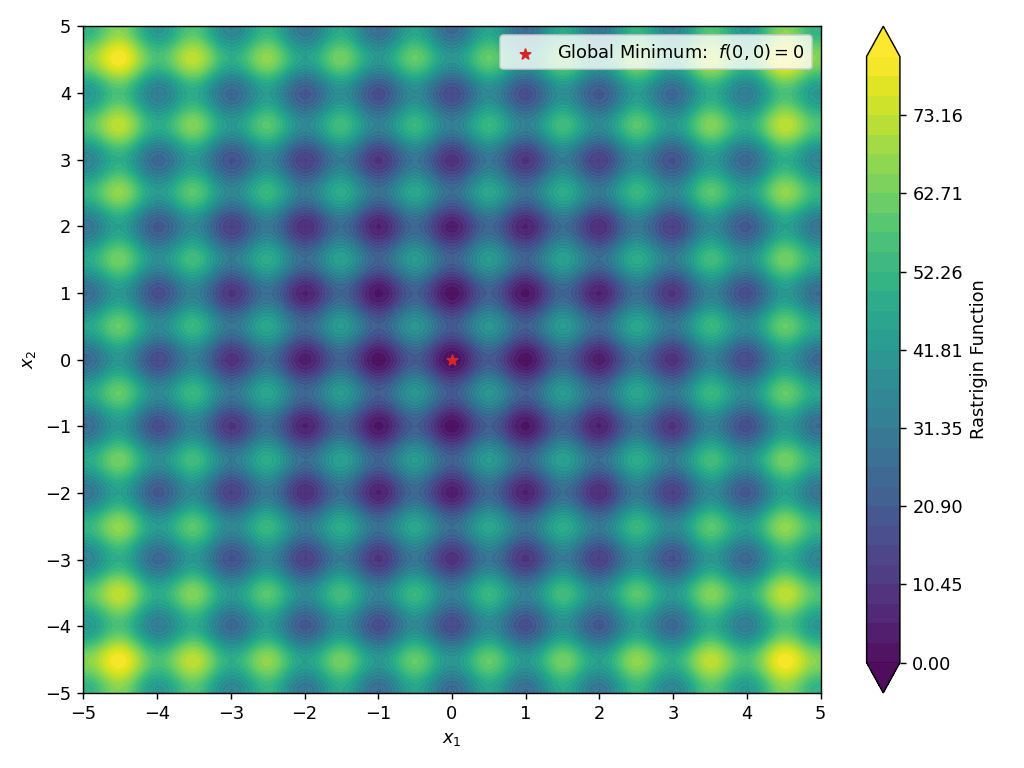
\includegraphics[width=0.5\textwidth]{benchmarks/test_Rastrigin.png}}
	\caption{The Rastrigin function.}
	\label{fig:Rastrigin}
\end{figure}

\begin{figure}[htbp]
	\centerline{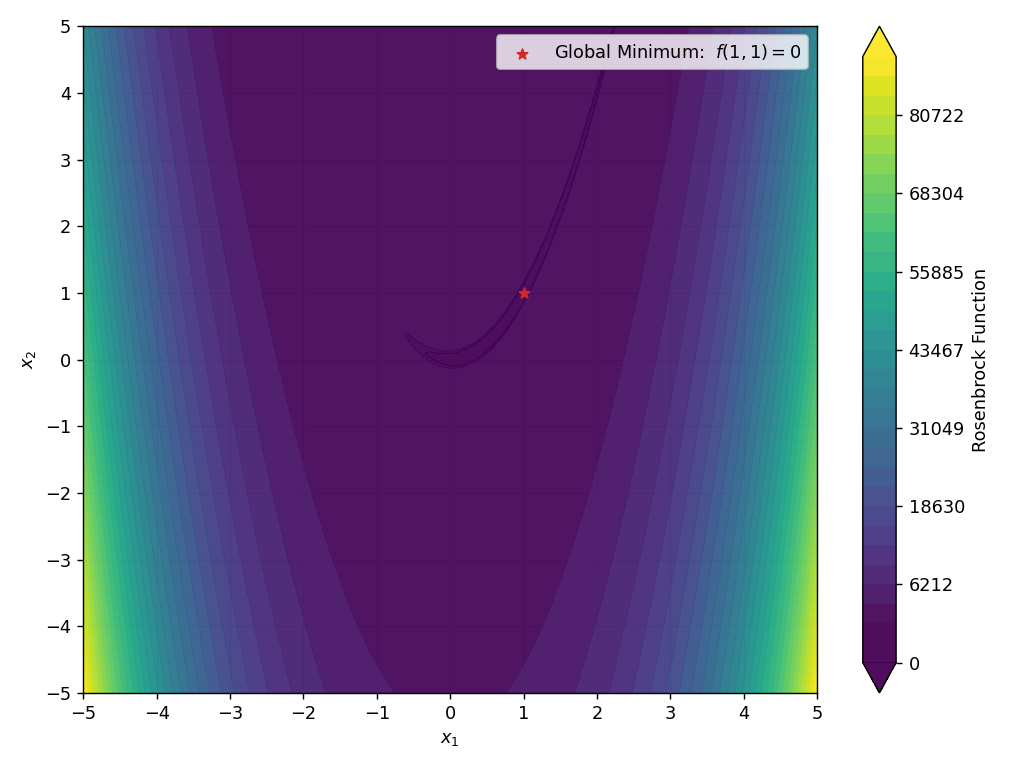
\includegraphics[width=0.5\textwidth]{benchmarks/test_Rosenbrock.png}}
	\caption{The Rosenbrock function.}
	\label{fig:Rosenbrock}
\end{figure}

\begin{figure}[htbp]
	\centerline{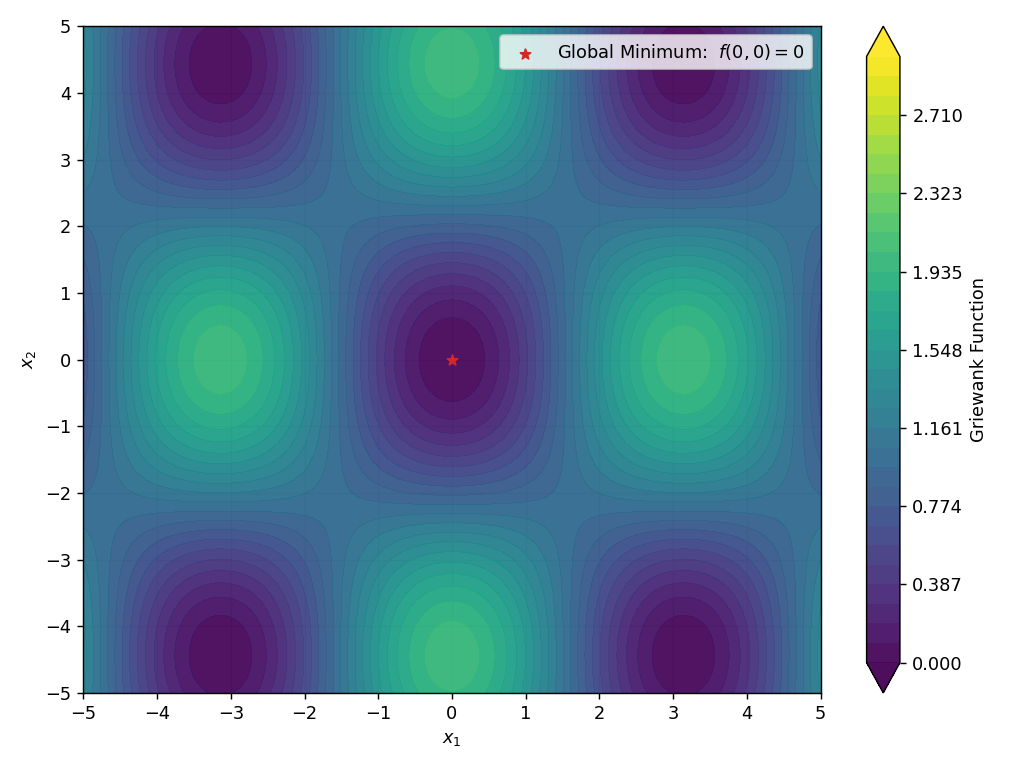
\includegraphics[width=0.5\textwidth]{benchmarks/test_Griewank.png}}
	\caption{The Griewank function.}
	\label{fig:Griewank}
\end{figure}

\begin{figure}[htbp]
	\centerline{\includegraphics[width=0.5\textwidth]{benchmarks/test_Styblinski–Tang.png}}
	\caption{The Styblinski–Tang function.}
	\label{fig:Styblinski–Tang}
\end{figure}

\subsubsection{Surrogate Model}

Given the ubiquity of machine learning surrogate models in the reviewed literature, this work adopts the same approach. In particular, a multilayer perceptron (MLP) with hidden layer architecture

$$ \left(\underbrace{100, 100, \cdots, 100}_{D\;\textrm{times}}\right) $$

\noindent that is, $D$ fully-connected layers of 100 neurons each, is adopted. Model training, validation, and testing are carried out using the functionalities of scikit-learn and PyTorch; for details, refer to the GitHub repo. That said, note that the loss function used in the course of training, validation, and testing is (\ref{eqn:surrogate_error}).

\subsubsection{Monte Carlo}

In order to test (\ref{eqn:efficiency_proposition}) and address question 2, a full factorial Monte Carlo approach is taken. This approach can be summarized in the following pseudocode:

\newpage
\begin{verbatim}
for benchmark_problem in benchmark_list:
  for sampling_scheme in scheme_list:
    for D in [2, 3, 4, 5, 6]:
      for N in [
      	3D, 4D, 5D, ..., 10D,
      	3^D, 4^D, 5^D, ..., 10^D
      ] up to max of 10^5:
        for trial = 1 ... 50:
          sample objective, get data;
      
          train/test split data;
      
          normalize data;
      
          train surrogate using
            validation/early-stopping;
        
          test surrogate;
        
          compute surrogate efficiency
            using test data;
        
          log results;
\end{verbatim}

\noindent That is, for every combination of benchmark problem, sampling scheme, dimensionality, and number of samples, do 50 Monte Carlo trials of sample (some randomness here), split (some randomness here), train (some randomness here), and test. By way of this approach, a results table with up to $4\times 2\times 5\times 16\times 50 = 32,000$ rows is generated. Note that the ``\texttt{up to max of 10\^{}5}" limit placed on number of samples (for the sake of runtime) is why the results table contains \textit{up to} 32,000 rows; the actual number obtained will be less than this.

\section{Results}

The described full factorial Monte Carlo approach was carried out, and 30,800 rows of data were ultimately obtained. The scripts, data, and all visualizations are available on the GitHub repo. Figures \ref{fig:Rastrigin_results_simple_random} - \ref{fig:Styblinski-Tang_results_latin_hypercube} show a selection of results, namely the $\mathbb{R}^4\to\mathbb{R}$ cases for each benchmark and sampling scheme.

\begin{figure}[htbp]
	\centerline{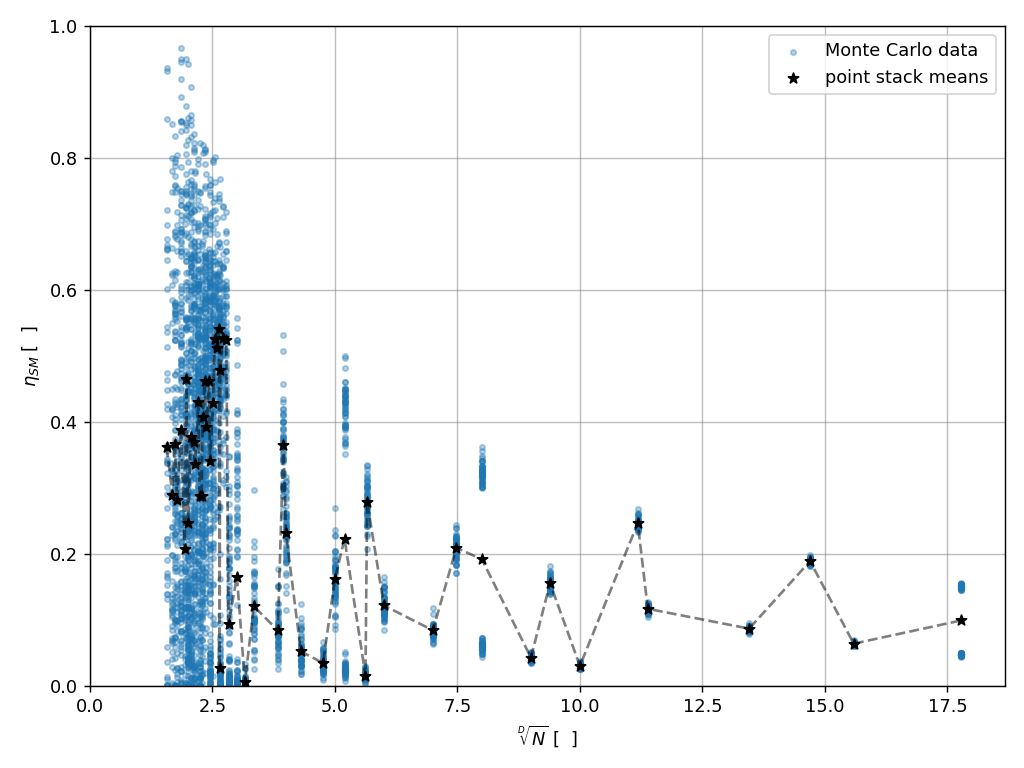
\includegraphics[width=0.5\textwidth]{results/rastrigin/results_sampling_simple_random_dimensionality_4.png}}
	\caption{Results for the Rastrigin function ($\mathbb{R}^4\to\mathbb{R}$) under simple random sampling.}
	\label{fig:Rastrigin_results_simple_random}
\end{figure}

\begin{figure}[htbp]
	\centerline{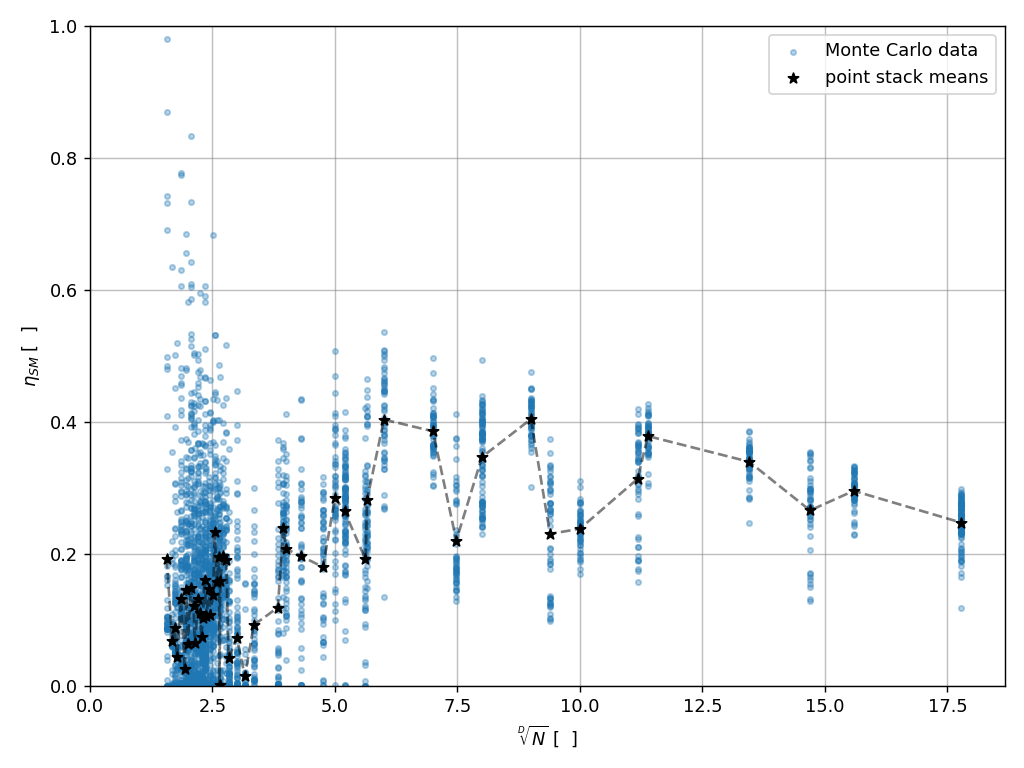
\includegraphics[width=0.5\textwidth]{results/rosenbrock/results_sampling_simple_random_dimensionality_4.png}}
	\caption{Results for the Rosenbrock function ($\mathbb{R}^4\to\mathbb{R}$) under simple random sampling.}
	\label{fig:Rosenbrock_results_simple_random}
\end{figure}

\begin{figure}[htbp]
	\centerline{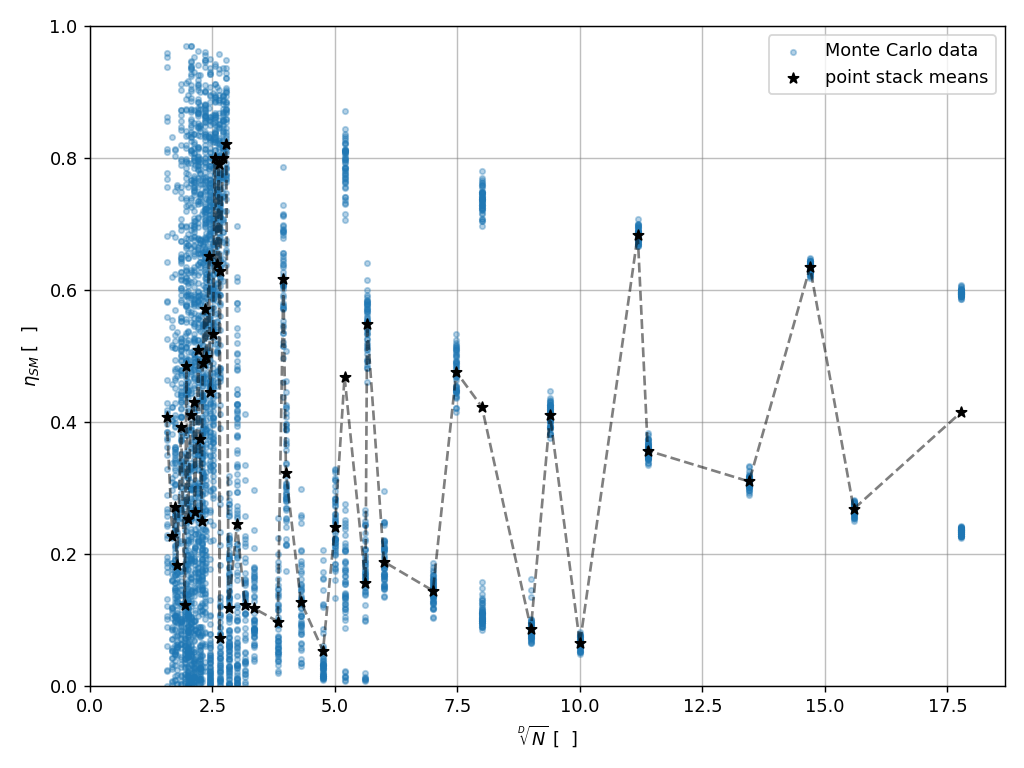
\includegraphics[width=0.5\textwidth]{results/griewank/results_sampling_simple_random_dimensionality_4.png}}
	\caption{Results for the Griewank function ($\mathbb{R}^4\to\mathbb{R}$) under simple random sampling.}
	\label{fig:Griewank_results_simple_random}
\end{figure}

\begin{figure}[htbp]
	\centerline{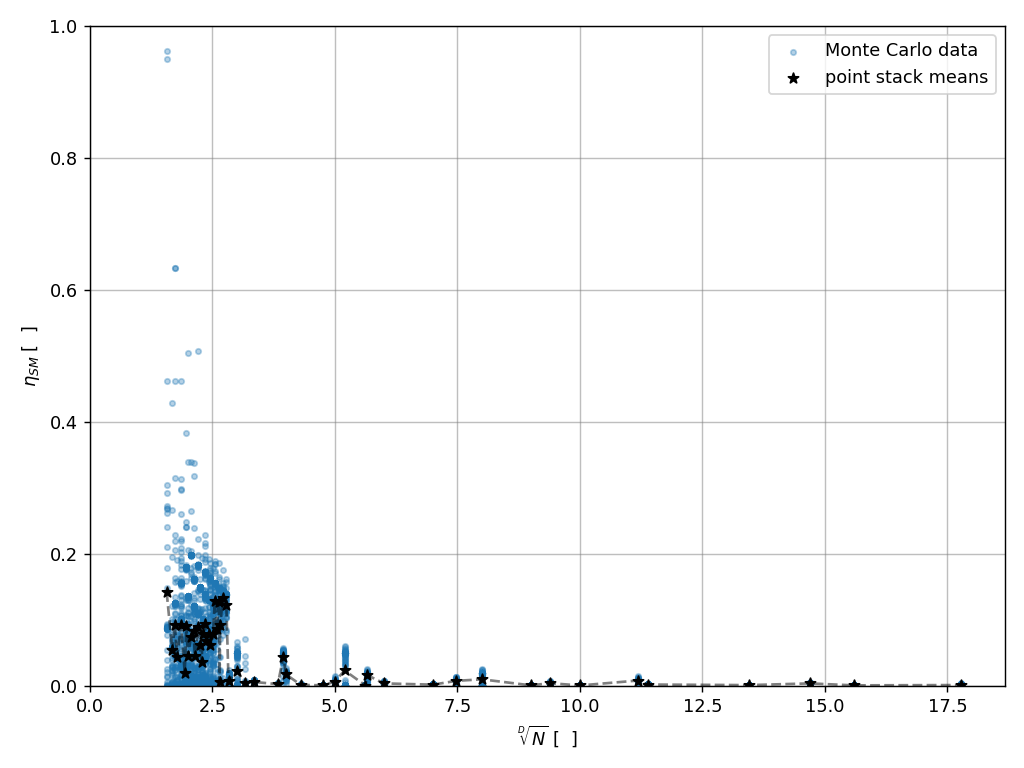
\includegraphics[width=0.5\textwidth]{results/styblinskitang/results_sampling_simple_random_dimensionality_4.png}}
	\caption{Results for the Styblinski-Tang function ($\mathbb{R}^4\to\mathbb{R}$) under simple random sampling.}
	\label{fig:Styblinski-Tang_results_simple_random}
\end{figure}

\begin{figure}[htbp]
	\centerline{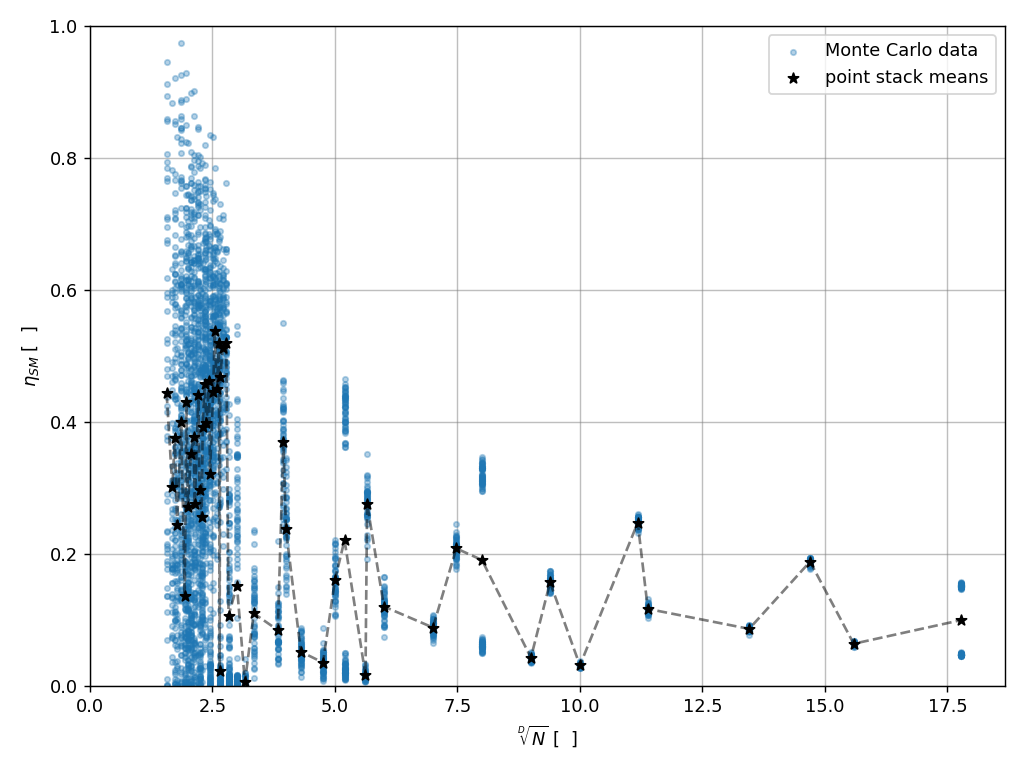
\includegraphics[width=0.5\textwidth]{results/rastrigin/results_sampling_latin_hypercube_dimensionality_4.png}}
	\caption{Results for the Rastrigin function ($\mathbb{R}^4\to\mathbb{R}$) under latin hypercube sampling.}
	\label{fig:Rastrigin_results_latin_hypercube}
\end{figure}

\begin{figure}[htbp]
	\centerline{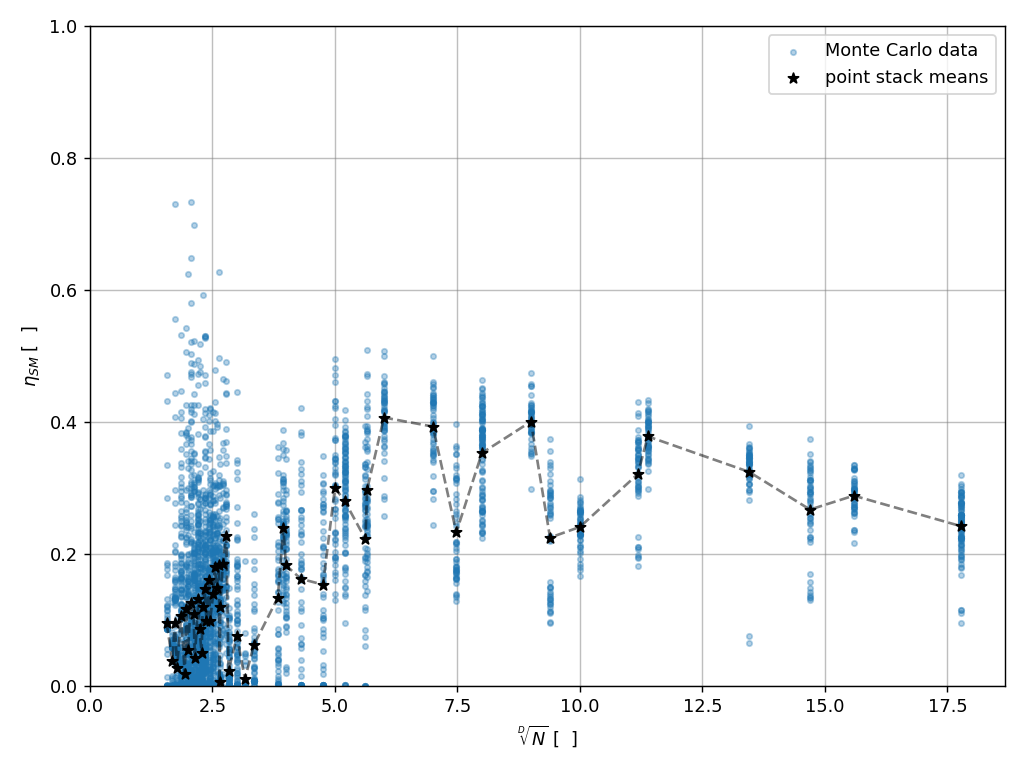
\includegraphics[width=0.5\textwidth]{results/rosenbrock/results_sampling_latin_hypercube_dimensionality_4.png}}
	\caption{Results for the Rosenbrock function ($\mathbb{R}^4\to\mathbb{R}$) under latin hypercube sampling.}
	\label{fig:Rosenbrock_results_latin_hypercube}
\end{figure}

\begin{figure}[htbp]
	\centerline{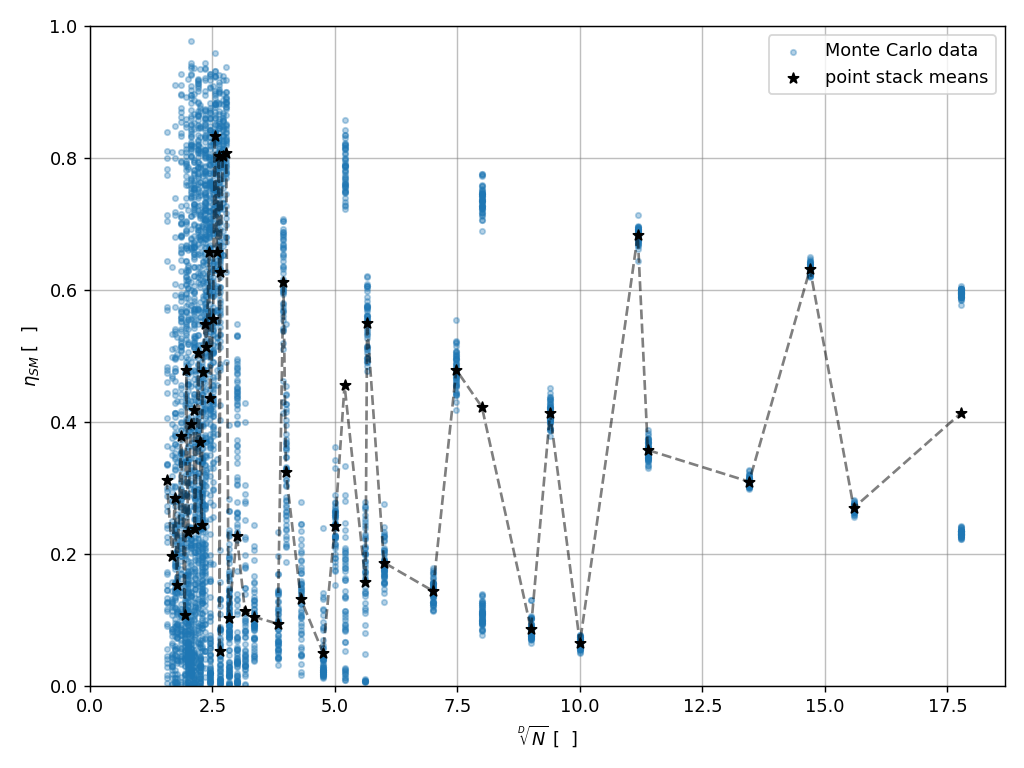
\includegraphics[width=0.5\textwidth]{results/griewank/results_sampling_latin_hypercube_dimensionality_4.png}}
	\caption{Results for the Griewank function ($\mathbb{R}^4\to\mathbb{R}$) under latin hypercube sampling.}
	\label{fig:Griewank_results_latin_hypercube}
\end{figure}

\begin{figure}[htbp]
	\centerline{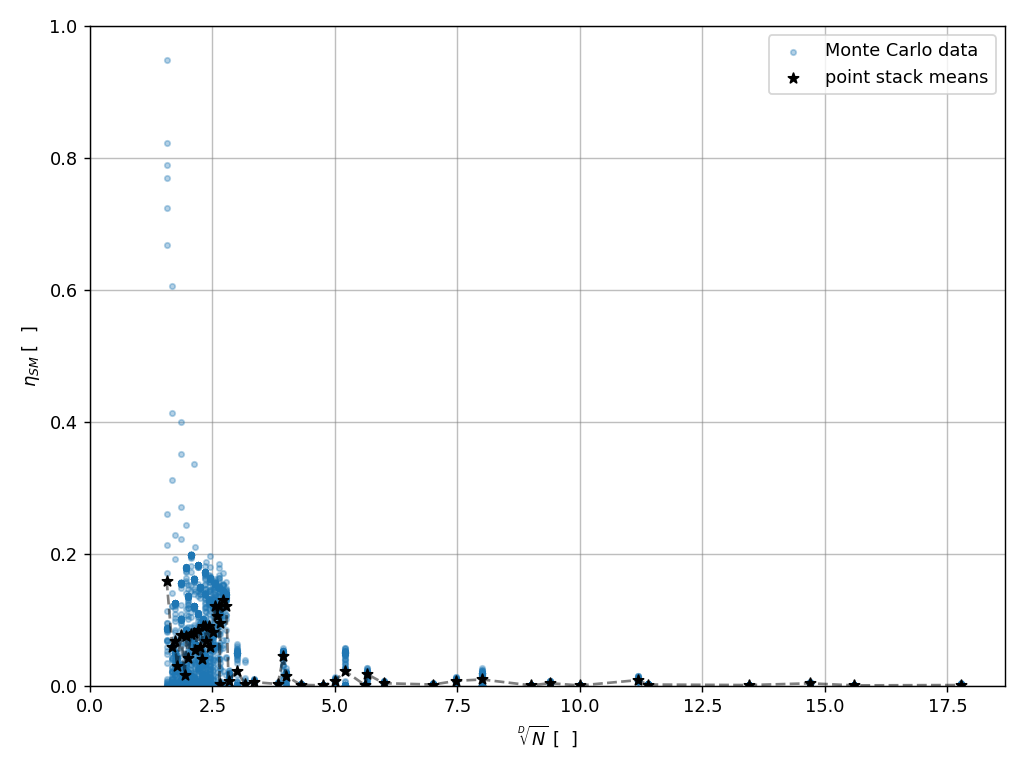
\includegraphics[width=0.5\textwidth]{results/styblinskitang/results_sampling_latin_hypercube_dimensionality_4.png}}
	\caption{Results for the Styblinski-Tang function ($\mathbb{R}^4\to\mathbb{R}$) under latin hypercube sampling.}
	\label{fig:Styblinski-Tang_results_latin_hypercube}
\end{figure}

\section{Discussion}

An inspection of Figures \ref{fig:Rastrigin_results_simple_random} - \ref{fig:Styblinski-Tang_results_latin_hypercube} reveals a few expected results. First, there is a high degree of variance within the Monte Carlo trials of a given sample size for small samples, with the variance tending to decrease as sample size increases. There are also noticeable differences between the simple random sampling results and the latin hypercube results for small samples. Beyond a certain sample size, however, the results appear similar for both sampling schemes.

An inspection of Figures \ref{fig:Rastrigin_results_simple_random} - \ref{fig:Styblinski-Tang_results_latin_hypercube} also reveals a few interesting results. If one ignores the high variance region associated with small sample sizes, the surrogate efficiency for Rastrigin seems to attain a maximum around $\sqrt[D]{N} = 4$. Similarily, for Rosenbrock it appears to be around $\sqrt[D]{N} = 6$, and for Griewank it appears to be around $\sqrt[D]{N} = 11$. For Styblinski-Tang, it appears to be around $\sqrt[D]{N} = 4$ or 5, but the surrogate efficiency for this model also appears to be quite low across the range of sample sizes considered (thus suggesting that the choice of surrogate model architecture was a poor one for the Styblinski-Tang use case).

Conversely, if one includes the high variance regions associated with small sample sizes, then for the cases of Rastrigin, Griewank, and Styblinski-Tang a number of the small-sample point stack means are greater than, or equal to, the corresponding large-sample point stack means. This indicates that surrogate modelling by way of ensemble methods (with each ensemble member being a small-sample surrogate) is particularly applicable to these use cases. Only the Rosenbrock case appears to buck this trend. That is to say, it is evidently better to use a single, large-sample surrogate for Rosenbrock.

\section{Conclusion}

Recall the questions that this work set out to address; namely

\begin{enumerate}
	\item Is there a general metric for surrogate efficiency?
	\item []
	\item Is there a clear ``winner", with respect to surrogate efficiency, in terms of sampling scheme?
\end{enumerate}

Given the interesting results obtained, the proposed surrogate efficiency metric appears to behave in an ideal way. That is to say, it seems to work well over the set of benchmark problems chosen (i.e., it is general), and in each case it suggested an optimal sample size for a given benchmark, dimensionality, and sampling scheme (i.e., it is useful as a performance metric). Therefore, the answer to question 1 is yes (and the expression proposed in (\ref{eqn:efficiency_proposition}) seems to serve as a general metric).

As for question 2, the answer is most likely no. For smaller sample sizes, the point stack means tend to exhibit less variance in the latin hypercube case than in the simple random sampling case, but the actual surrogate efficiency values obtained are very similar in both cases. In addition, as was previously observed, past a certain sampling size the sampling scheme had no discernible impact upon surrogate efficiency.

\section{Future Work}

In reviewing the methodology and results of this work, it seems that the choice of $\sqrt[D]{N}$ in (\ref{eqn:efficiency_proposition}), while motivated by the consensus that problems increase in difficulty as their dimensionality increases (the so-called ``curse of dimensionality"), may have overestimated the degree to which difficulty increases in the number of dimensions. Therefore, rather than assuming that every problem difficulty scales like $\mathcal{O}(2^D)$, it would be more general to allow for problems to scale in various ways such as, for example, $\mathcal{O}(D^2)$ or $\mathcal{O}(D\log_2(D))$. This then suggests alternate expressions for surrogate efficiency such as 

\newpage
\begin{equation}
	\eta_\textrm{SM} = \exp\left[-\frac{N}{D^2}\left(\mu_\textrm{d-APE} + \textrm{IQR}_\textrm{d-APE}\right)\right]
	\label{eqn:efficiency_proposition_2}
\end{equation}

\noindent or

\begin{equation}
	\eta_\textrm{SM} = \begin{cases}
		\exp\left[-N\left(\mu_\textrm{d-APE} + \textrm{IQR}_\textrm{d-APE}\right)\right] & \textrm{if}\;\;D=1 \\
		{} & {} \\
		\exp\left[-\frac{N}{D\log_2(D)}\left(\mu_\textrm{d-APE} + \textrm{IQR}_\textrm{d-APE}\right)\right] & \textrm{otherwise}
	\end{cases}
	\label{eqn:efficiency_proposition_3}
\end{equation}

\noindent This then implies the following future work: experiment with modifying (\ref{eqn:efficiency_proposition}) and updating the full factorial Monte Carlo design to suit. For instance, consider changing the sampling size approach to something like

\begin{verbatim}
	for N in [
	    3D, 4D, ..., 20D,
	    3Dlog2(D), 4Dlog2(D), ..., 20Dlog2(D),
	    3D^2, 4D^2, 	..., 20D^2
	]
\end{verbatim}


%%%% ==== REFERENCES ================================================================ %%%%

\bibliography{/home/primed-anthony/MECH_PhD/tex/refs/refs.bib}{}
\bibliographystyle{IEEEtran}

\end{document}


%%%% ==== TEMPLATES ================================================================= %%%%

\begin{table}[htbp]
	\caption{Table Type Styles}
	\begin{center}
	\begin{tabular}{|c|c|c|c|}
		\hline
		\textbf{Table}&\multicolumn{3}{|c|}{\textbf{Table Column Head}} \\
		\cline{2-4} 
		\textbf{Head} & \textbf{\textit{Table column subhead}}& \textbf{\textit{Subhead}}& 		\textbf{\textit{Subhead}} \\
		\hline
		copy& More table copy$^{\mathrm{a}}$& &  \\
		\hline
		\multicolumn{4}{l}{$^{\mathrm{a}}$Sample of a Table footnote.}
	\end{tabular}
	\label{tab1}
	\end{center}
\end{table}

\begin{figure}[htbp]
	\centerline{
\includegraphics{fig1.png}}
	\caption{Example of a figure caption.}
	\label{fig}
\end{figure}
